\documentclass[a4paper,10pt]{article}
% Please adjust the data of your team and team members below

\def\teamnumber{00} % Enter the number of your team from Blackboard
\def\teamname{The Data Scientists} % Choose a creative name for your team
\def\teammemberAname{Jane Doe} % For each member, create such
\def\teammemberAstudentid{0123456}
\def\teammemberBname{John Roe}
\def\teammemberBstudentid{9876543}
\def\teammemberCname{Jane Roe}
\def\teammemberCstudentid{0123456}
\def\teammemberDname{John Doe}
\def\teammemberDstudentid{9876543}
\def\teammemberEname{Jane Modaal}
\def\teammemberEstudentid{0123456}
\def\teammemberFname{John Modaal}
\def\teammemberFstudentid{9876543}
\def\teammemberGname{Jep Doe Roe} % If you have six members, comment out with %
\def\teammemberGstudentid{1111111} % If you have six members, comment out with %

% This file contains a few packages and scripts

\usepackage[utf8]{inputenc}
\usepackage{subcaption}
\usepackage[english]{babel}
\usepackage{graphicx}
\usepackage{amssymb}
\usepackage{amsfonts}
\usepackage{amsmath}
\usepackage{multirow}
\usepackage{todonotes}
\usepackage{tabularx}
\usepackage{booktabs}

\usepackage{wrapfig} % for wrapping text around figures, use \begin{wrapfigure}[lineheight]{position}{width}

\usepackage{hyperref}
\hypersetup{backref,pdfborder=0 0 0} 
\urlstyle{sf}

\usepackage[par]{kantlipsum} % par or nopar

\newcommand{\teammembers}[2]{
  \ifdefined\teammemberGname
    \teammemberAname~ #1(\textit{\teammemberAstudentid}) #2
    \teammemberBname~ #1(\textit{\teammemberBstudentid}) #2  
    \teammemberCname~ #1(\textit{\teammemberCstudentid}) #2
    \teammemberDname~ #1(\textit{\teammemberDstudentid}) #2
    \teammemberEname~ #1(\textit{\teammemberEstudentid}) #2
    \teammemberFname~ #1(\textit{\teammemberFstudentid}) #2
    \teammemberGname~ #1(\textit{\teammemberGstudentid}) #2
  \else
    \teammemberAname~ #1(\textit{\teammemberAstudentid}) #2
    \teammemberBname~ #1(\textit{\teammemberBstudentid}) #2  
    \teammemberCname~ #1(\textit{\teammemberCstudentid}) #2
    \teammemberDname~ #1(\textit{\teammemberDstudentid}) #2
    \teammemberEname~ #1(\textit{\teammemberEstudentid}) #2
    \teammemberFname~ #1(\textit{\teammemberFstudentid}) #2
  \fi
}
\def\thedoc{Final Report}
\def\thestrategy{Strategy \& Concept}
\def\theproject{Practical Team Project}
\def\thecourse{Data Science and Society (INFOMDSS)}
\author{\teamname~(\teamnumber)}
\ifdefined\finalreport
  \def\plan{}
\else
  \def\plan{(Planned)}
\fi


\title{\thedoc}
\makeatletter
\begin{document}

  \thispagestyle{empty}

\begin{figure}[h]
    \vspace*{-2cm}
    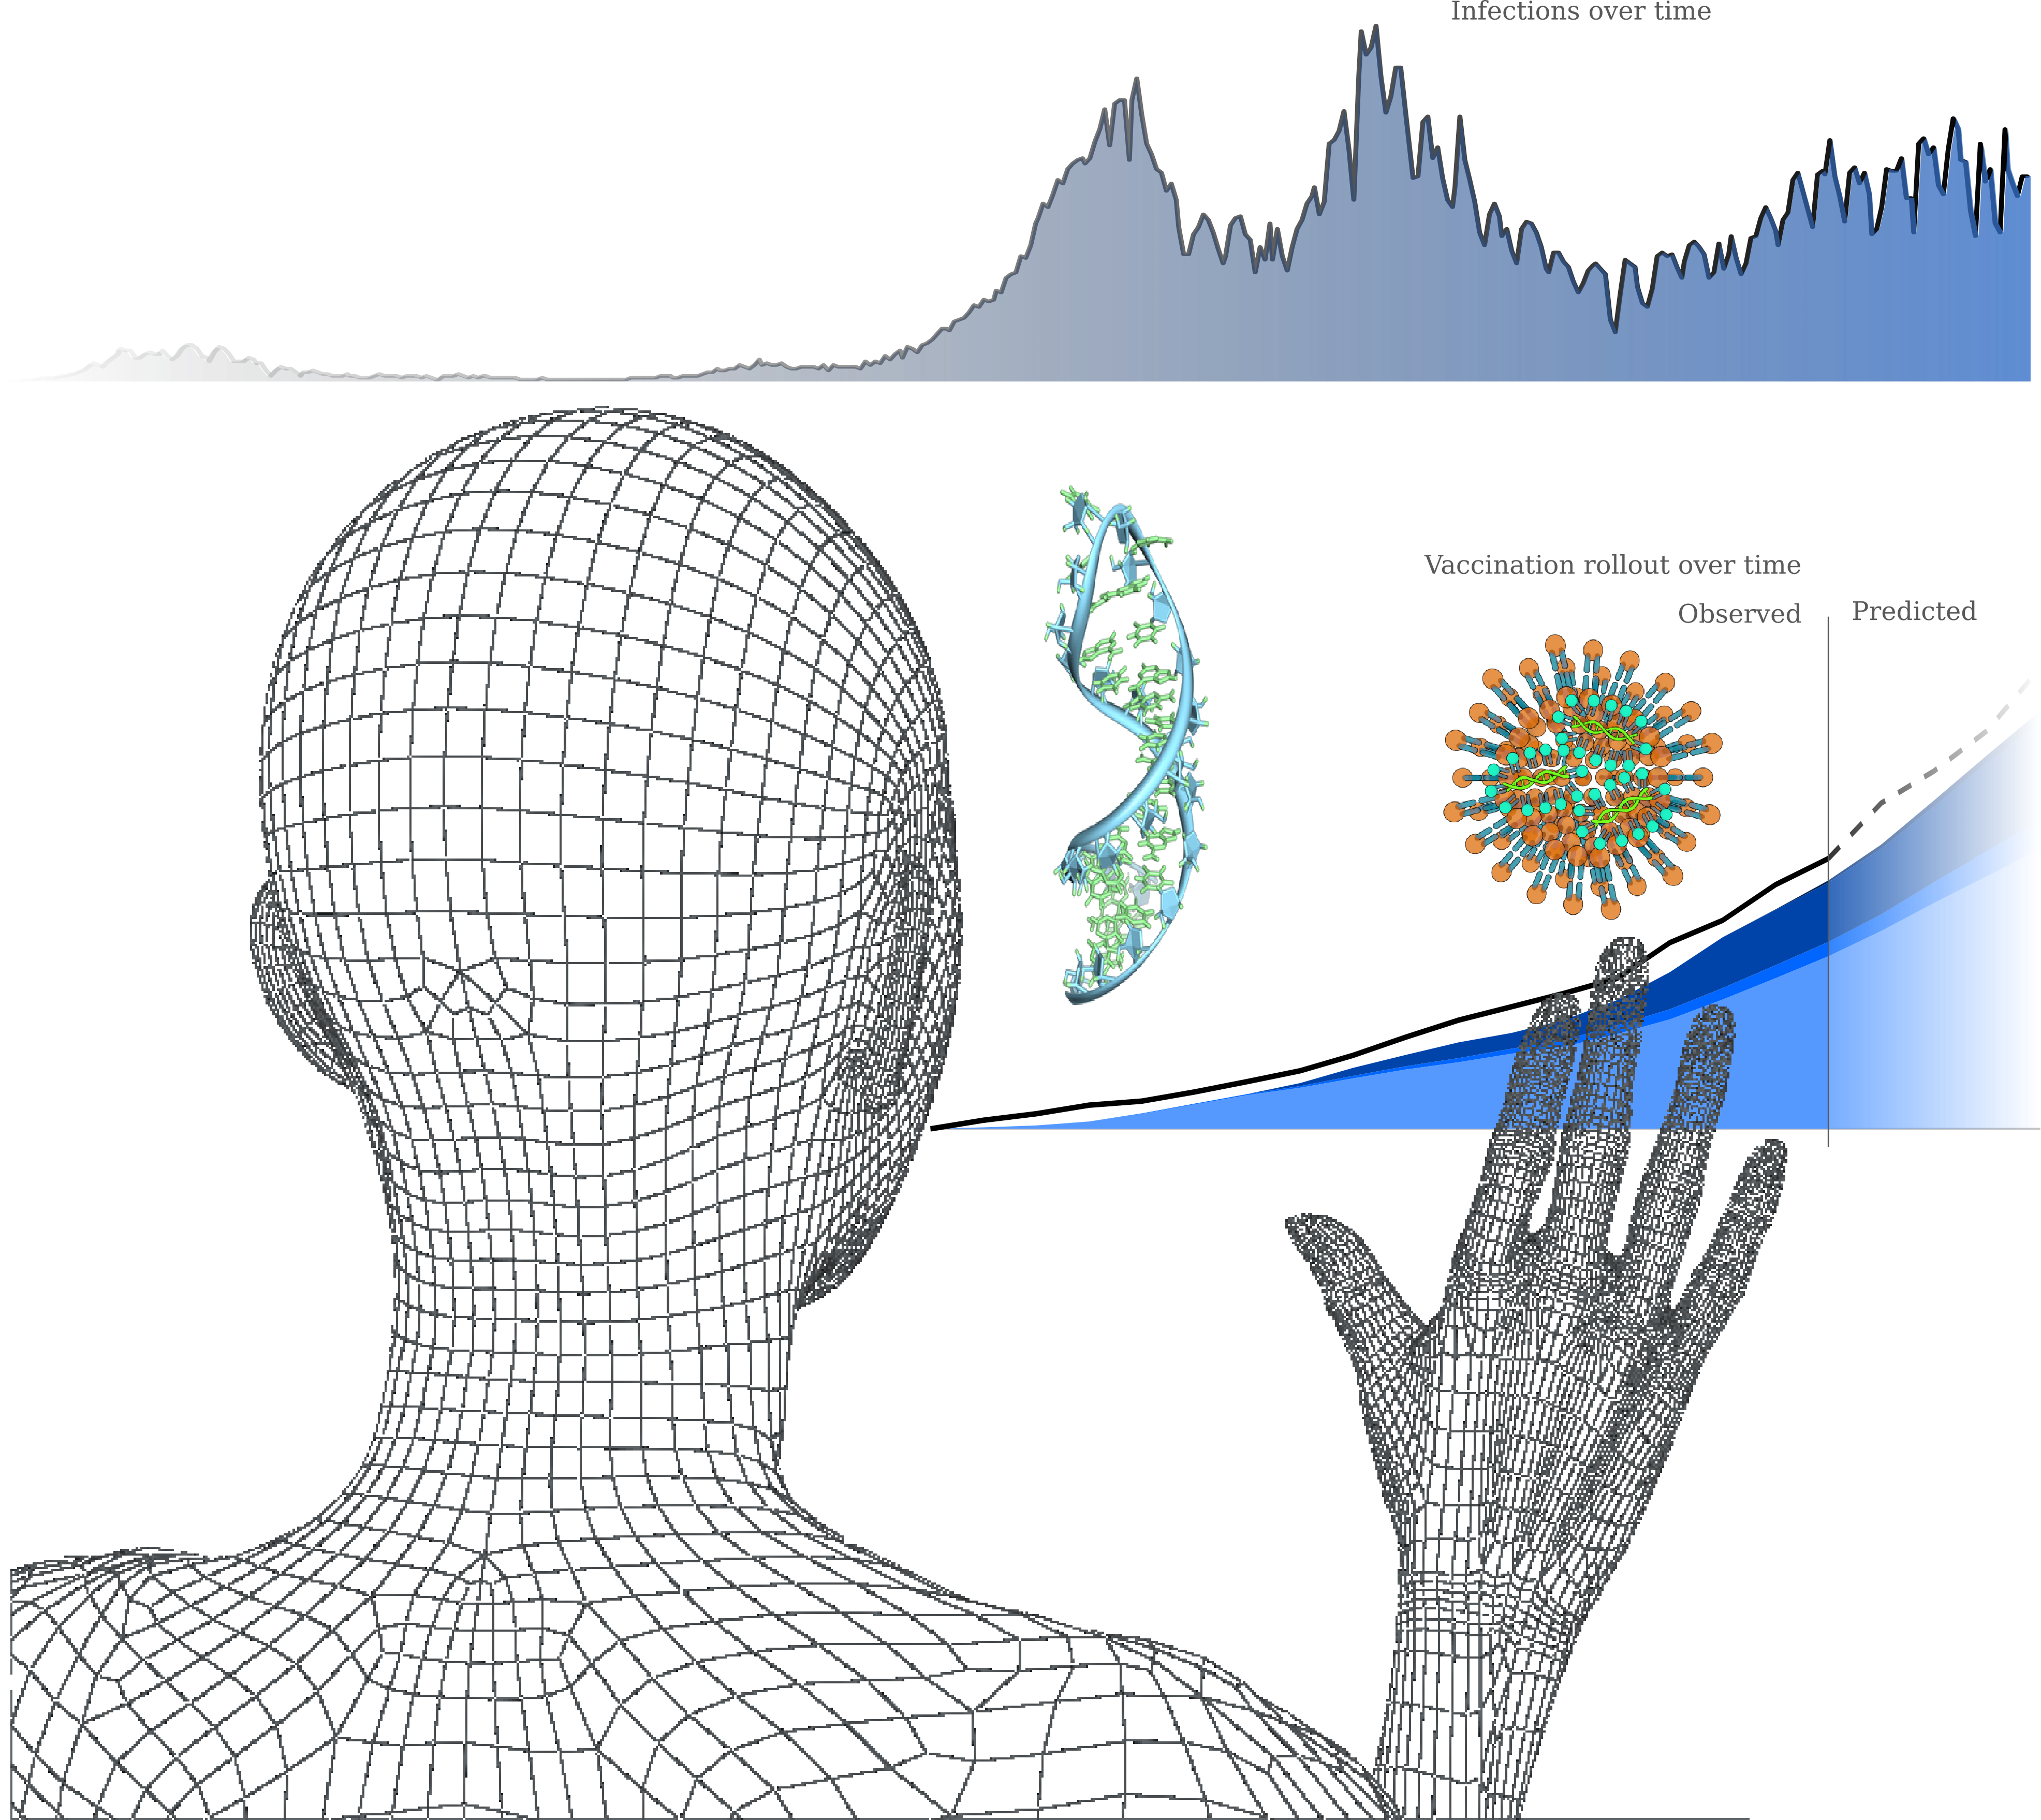
\includegraphics[width=\textwidth]{fig/datascience_covid_dashboard.png}
    \caption*{\tiny Source: 3D: G.Krempl. RNA,mRNA vaccine: Wikipedia Commons. Cases \& Vaccination NL: RIVM.}
\end{figure}
\vspace{2cm}
\begin{center}
  \textbf{\Huge \@title}
  \bigskip \\ by 
  \medskip \\
  \textbf{\large \@author}
  \bigskip \\
  \begin{tabular}{ll}
    \teammembers{&}{\\}
  \end{tabular}
\end{center}

The final report template formatted according to the requirements of INFOMDSS 2026-27.

\vfill

\begin{flushleft}
  \textbf{\large Utrecht University \hfill \today} 
\end{flushleft}

\pagebreak
\thispagestyle{empty}


\section*{Executive Summary}
% This input file is for your summary
Provide a 150-250 words summary here of the project entailing everything an abstract should entail. \\
\url{https://writing.wisc.edu/handbook/assignments/writing-an-abstract-for-your-research-paper/}


\tableofcontents 
%\listoffigures
%\listoftables

\clearpage \newpage \setcounter{page}{1}

\section{Business and Data Understanding} \label{sec:businessdataunderstanding}
\subsection{Aims and Scope}

Begin with introducing the problem and reasoning behind team's interest in building a dashboard in context of this problem. 

This section will summarize the objectives this dashboard aims to achieve. 

\subsubsection{Topic and targeted policymaker.}
Describe the main topic and policymaker you selected here

\paragraph{Context}
~\\ PLACEHOLDER: Netherlands Housing Market, American Housing Market, Changes in Housing Prices since 1950 etc. 

% \paragraph{Data included in the analysis:} 
% ~\\ Population in each street-level pincode in the Netherlands, Number of hospitals in each city, etc.

\subsubsection{Targeted stakeholders and identified information needs.}
Describe the stakeholders at the policymaker or business leadership level and their information needs.  

\subsubsection{Key Performance Indicators and Critical Success Factors}
Describe the KPIs and CSFs here aligned with the targeted stakeholders/information needs. The KPIs and CSFs need to be measurable and identifiable for the stakeholders such that it is actionable for a policymaker when being presented to them.

An example: 
\begin{table}[h]
\centering
\caption{CSF-to-KPI Mapping for Dashboard Design}
\begin{tabularx}{\textwidth}{l X X l}
\toprule
\textbf{CSF} & \textbf{KPI} & \textbf{Chart Type} & \textbf{Data Source}\\
\midrule
Customer retention & Monthly churn rate & Line chart (trend) & CRM export \\
Customer retention & Customer lifetime value & Bar chart by segment & Billing system \\
Customer retention & Repeat purchase rate & Line chart (trend) & Order database \\
\bottomrule
\end{tabularx}
\end{table}

\subsubsection{Our contribution.}
What you contribute \& how it creates value

\subsection{Related Projects and Dashboards}
In the first phase of the project, you must have gone through several publicly available dashboards and those mentioned in academic research. You can also search for similar projects in enterprise level that may have been mentioned in the media. Why are these dashboards good at what they do, why could they be useful for you, what could be improved and which gap remains after all the related projects. The following example highlights examples built in past few years to study the spread of Covid-19. 

The two most related dashboards to ours are the Confirmed Infections Dashboard by RIVM\footnote{\url{https://coronadashboard.government.nl}, retrieved \today.}, shown in Fig.~\ref{fig:reldashboards:1}, and the Confirmed Infections Dashboard by RIVM\footnote{\url{https://coronadashboard.government.nl}, retrieved \today.}, shown in Fig.~\ref{fig:reldashboards:2}. \todo{Replace by the 1-3 most related dashboards you found on the web.}

\begin{figure}[h!]
  \centering
  \begin{subfigure}{.49\textwidth}
    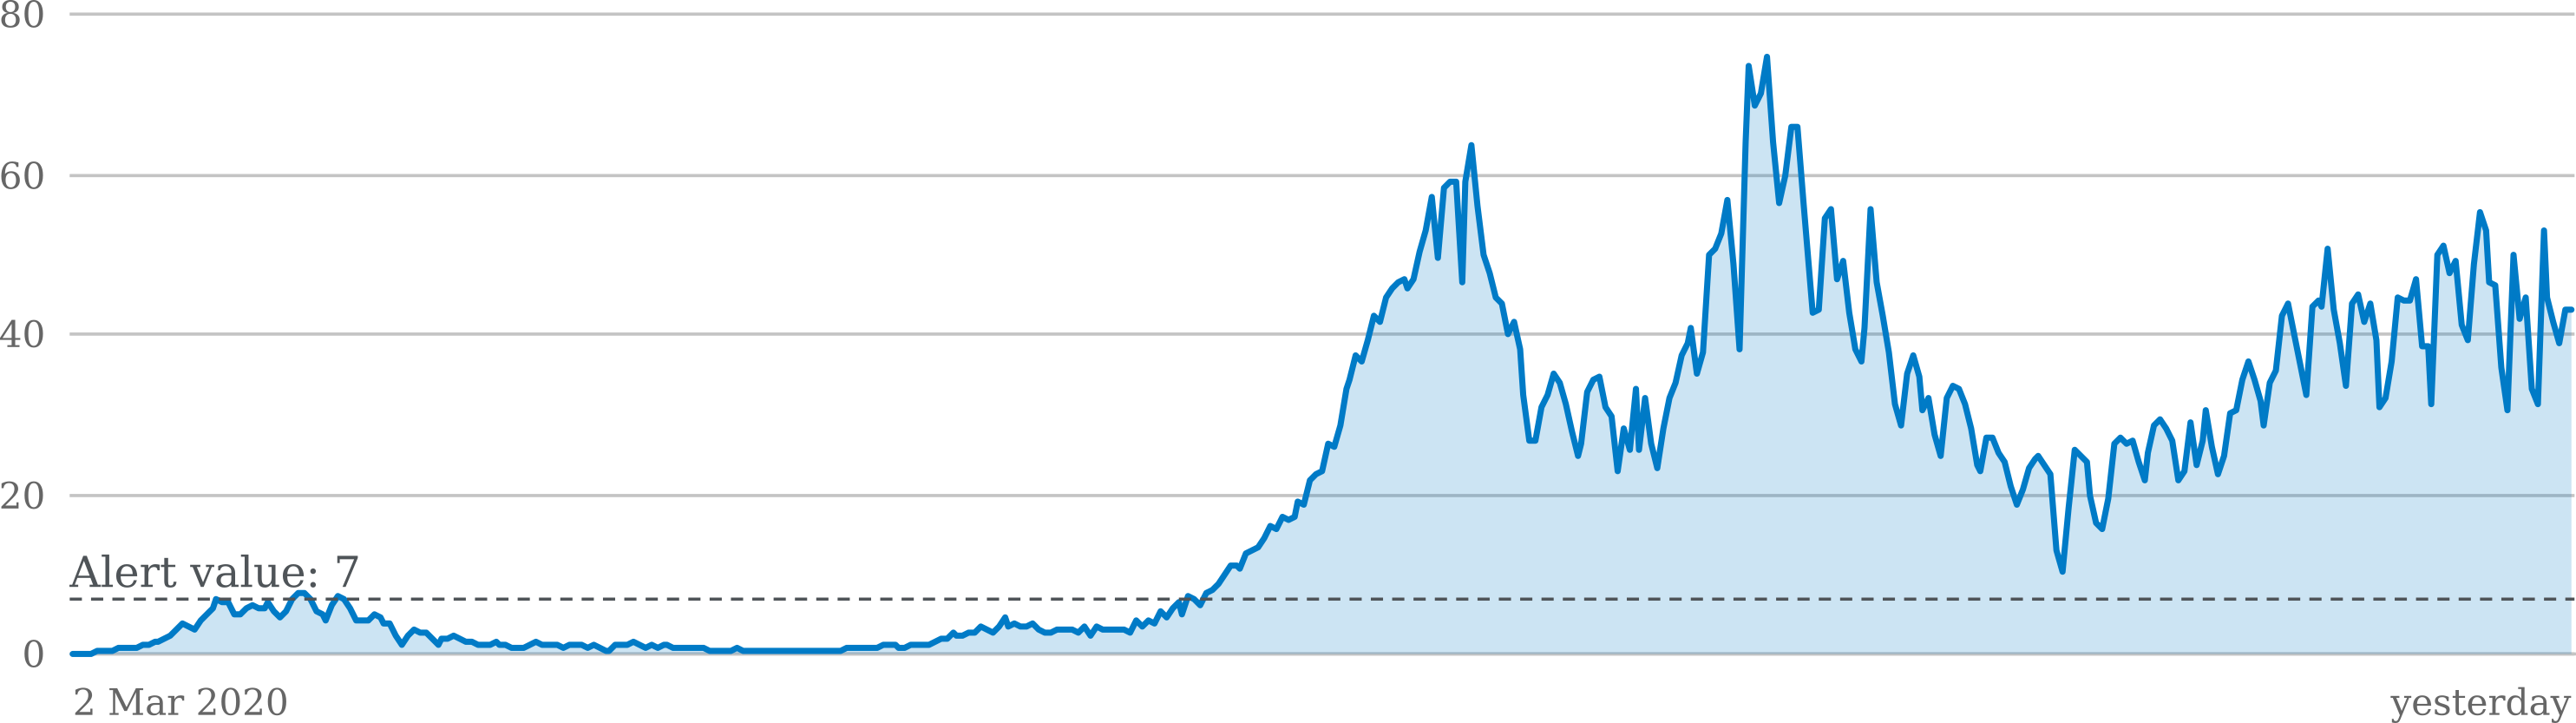
\includegraphics[width=\textwidth]{fig/infections_2021_may.png}
    \caption{RIVM Confirmed Infections}
    \label{fig:reldashboards:1}
  \end{subfigure}
  \begin{subfigure}{.49\textwidth}
    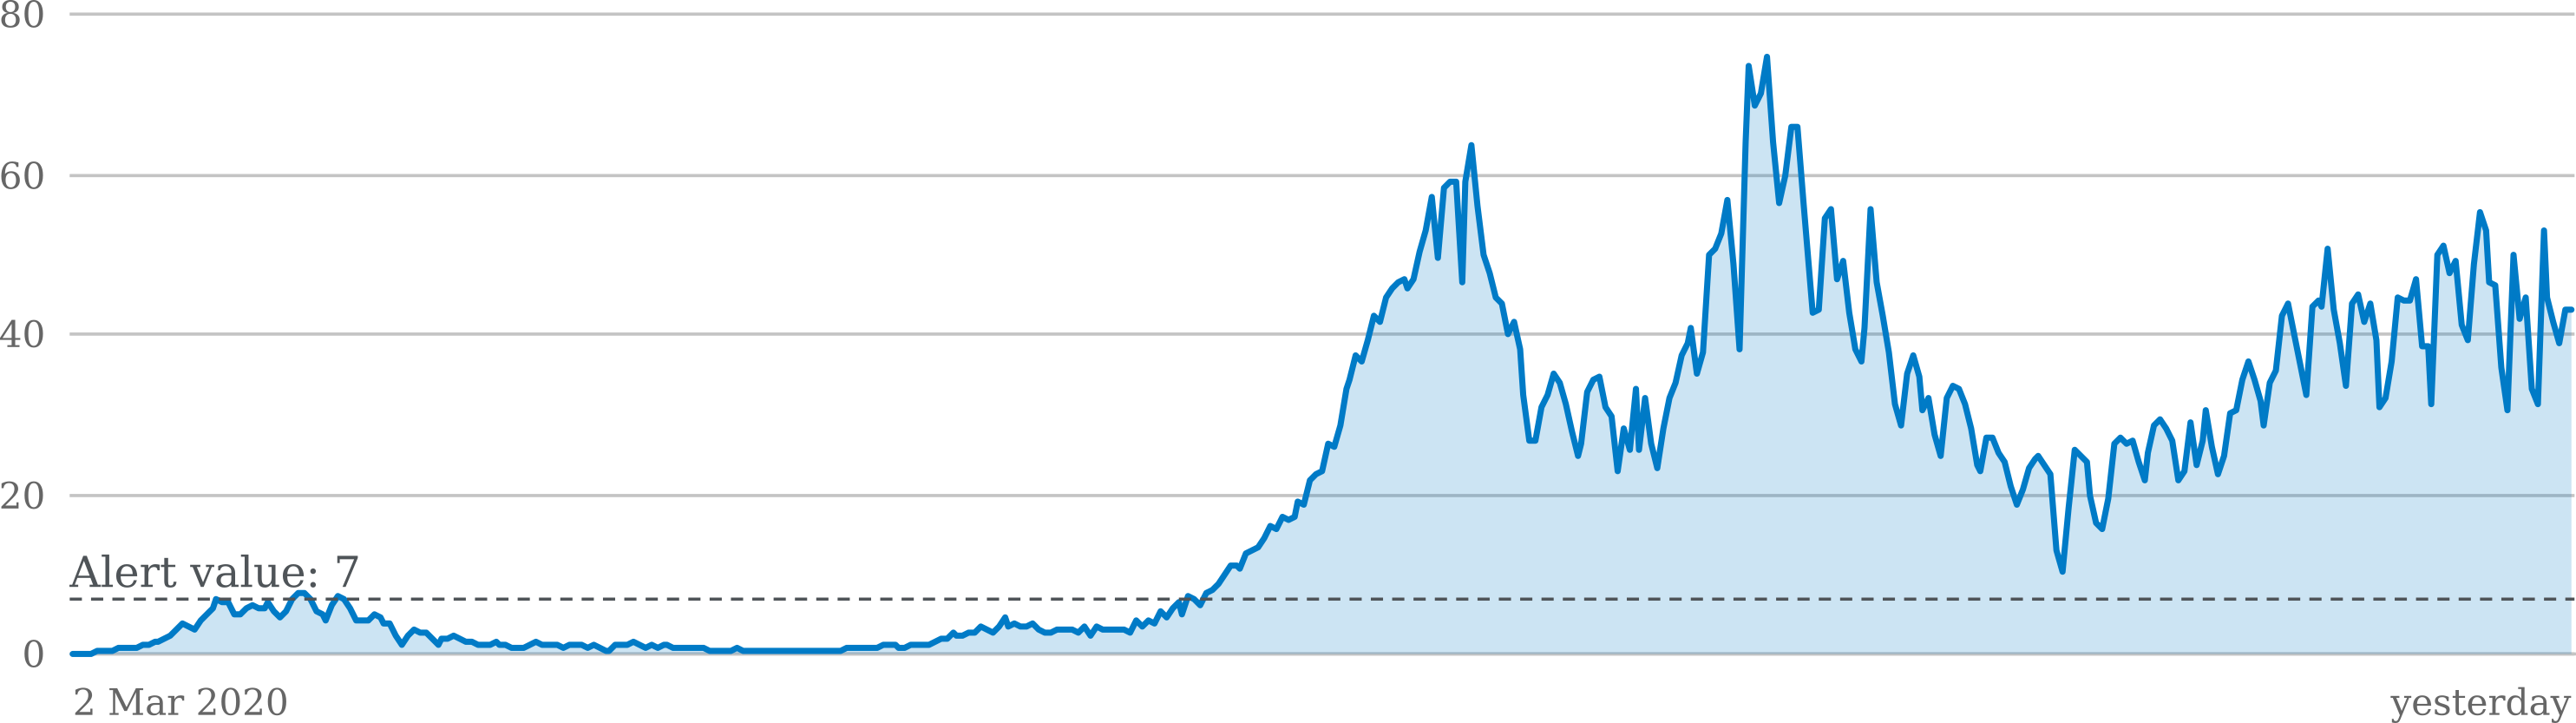
\includegraphics[width=\textwidth]{fig/infections_2021_may.png}
    \caption{RIVM Confirmed Infections}
    \label{fig:reldashboards:2}
  \end{subfigure}
  \caption{The most related dashboards.}
\end{figure}

\paragraph{RIVM Dashboard.}
Replace with your description

\paragraph{The other RIVM Dashboard.}
\footnote{\url{https://coronadashboard.government.nl}, retrieved \today.}
Replace with your description


\subsection{Summary of our Approach.}
Here, we provide a brief summary of our approach\todo{Edit: Summarise the \textbf{how} of your implementation}, before summarising the data sources, the analytics and visualisations, and the evaluation and deployment below. A mock-up / screenshot of our interactive dashboard is given in Fig.~\ref{fig:ourdashboard:1}-\ref{fig:ourdashboard:2}.

It is possible that your approach will change over time as you begin to explore more data sources and learn various methods in this course. This section would highlight your current plans. \\

For the \textbf{concept report}: This should entail your current plan on how to go about the data, visualisations and evaluation \& deployment just as written down here in the headers \\

For the \textbf{final submission}: This should entail an introduction on your methodology and data for the final part. Data Sources should be fully done in the data dictionary which is added as a seperate document, where here you just have to summarise the data that is used in the project. The analytics and visualisations should logically be in chapter 2, where here you just introduce it. The evaluation and deployment should logically be in chapter 3, where here you just introduce it. The headers below may be removed from Chapter 1, since they will be found elsewhere in the document. \\

\subsubsection{Data sources.}
Summarise the data sources and their integration, before they are described one-by-one. Note: The question ‘What is the format of the data?’ will be analysed in more detail under the Data Preparation and Modelling section which falls out of scope for the Concept Report. In this section, simply state the format (file type) and update frequency.
\todo[inline]{Enter a description for all your data sources here, including their relevance to the KPI. A good starting point for data sources on the Netherlands is: \url{https://data.rivm.nl/covid-19/}. When describing the data sources, please include the link to the data source.}
% \paragraph{Netherlands: RIVM COVID-19 Casus Landelijk}
% \begin{description}
%   \setlength\itemsep{0em}
%   \item[Scope:] Netherlands, daily infections cases with demographics and outcomes
%   \item[Source:] RIVM \url{https://data.rivm.nl/covid-19/COVID-19_casus_landelijk.html}
%   \item[License:] Open access, Public Domain Mark 1.0
%   \item[Format:] CSV, updated daily at 15:15
%   \item[Import:] Daily ETL
%   \item[Known issues:] Change (relaxation) of testing requirements on 2020-06-01.
% \end{description}

\subsubsection{Analytics and visualisation.}
“Describe which analytics and visualisations will be implemented, what information they will present, and which of them will be interactive.”
\begin{figure}[h]
  \centering
  \begin{subfigure}{.49\textwidth}
    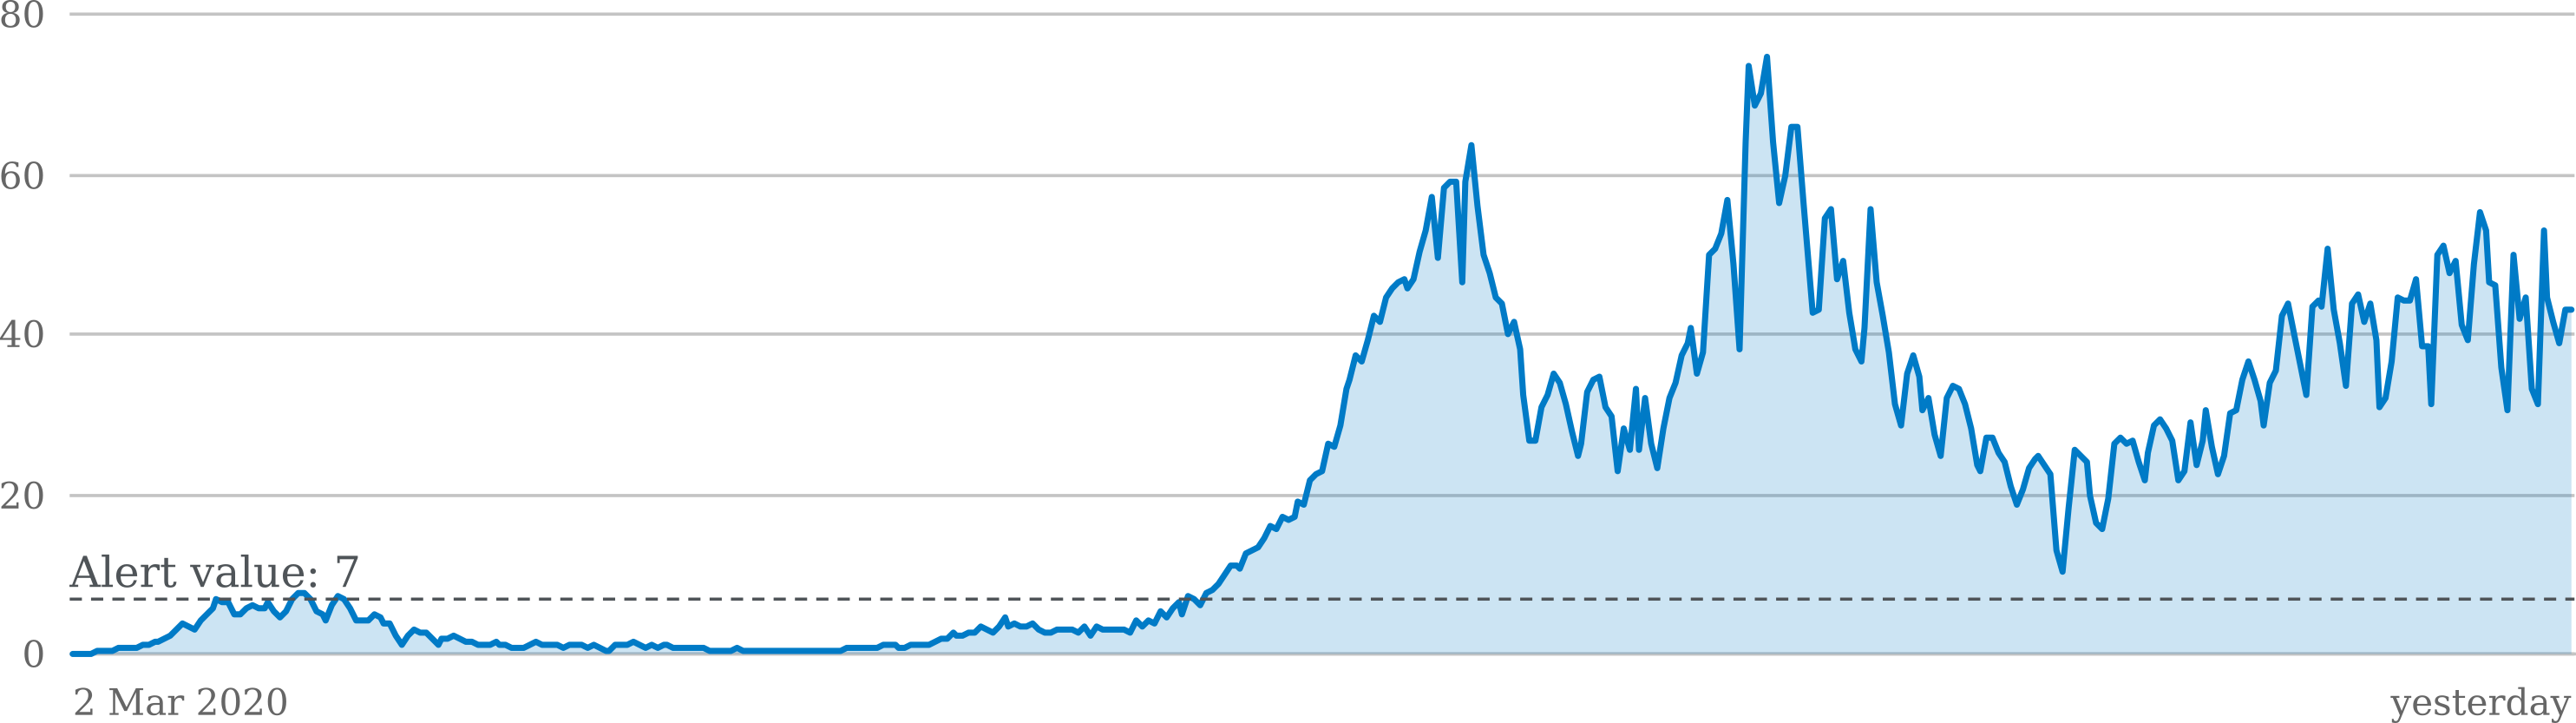
\includegraphics[width=\textwidth]{fig/infections_2021_may.png}
    \caption{View 1}
    \label{fig:ourdashboard:1}
  \end{subfigure}
  \begin{subfigure}{.49\textwidth}
    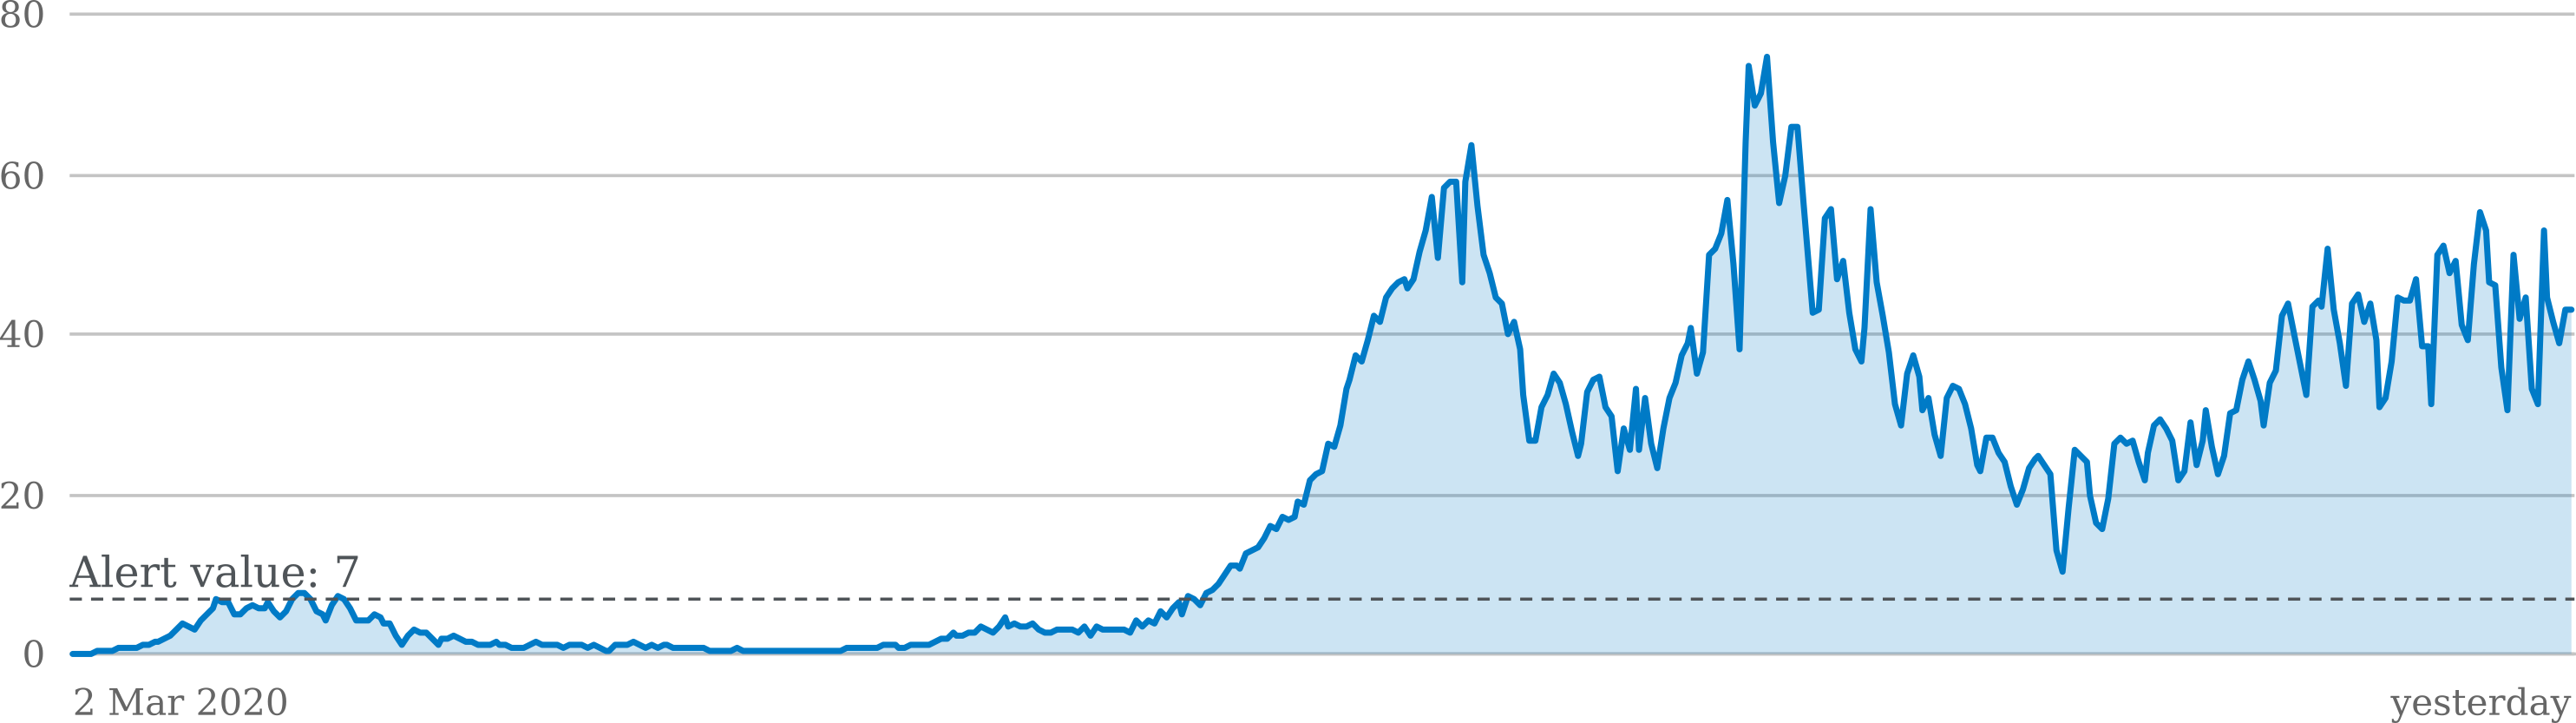
\includegraphics[width=\textwidth]{fig/infections_2021_may.png}
    \caption{View 2}
    \label{fig:ourdashboard:2}
  \end{subfigure}
  \caption{Mock-up of our dashboard.}
\end{figure}

\subsection{Planned Evaluation and Deployment.}

\subsubsection{Criteria of success and evaluation.}
Criteria, evaluation plan
I.e. when is the dashboard succesful for a stakeholder? When is it good for the policymaker? What are shortcomings and future plans for the dashboard etc. This list is not exhaustive, just an example. Please add onto it what the team finds necessary. 

\subsubsection{Deployment and maintenance.}
Needs for deployment \& maintenance 
An example: \url{https://medium.com/@amarakoonanjalee11/understanding-sdlc-deployment-maintenance-the-final-phase-d2a6b26cf9e0} 
\\
\textbf{Do not make any assumptions! I.e. an uptime of 99\% should be motivated why it is necessary. An uptime of 99\% as-is is not feasible if the computing power required is a lot or when the dashboard is only used once-twice a month. If you do not know the situation at the policymaker, tell us how they can make this dashboard succesful, deployable and maintainable for the future.} \\ \\
At this point the concept report stops and has reached a maximum of 4 pages excluding the front page, contents and  Appendix. Do not include the hours logged.



\section{Data Preparation and modelling} \label{sec:dataprepmodelling} 
\subsection{Data Preparation.}

\begin{itemize}
  \item What is the format of the data?
  \begin{itemize} 
    \item Is it static, time-series or streaming data?
    \item How many instances are there?
    \item Is the data representative, or is there a bias?
    \item What structure does the data have?
    \item Which variables are there, what do they represent, 
      \\ what is their type/encoding?
    \item Are there obvious data problems?
      \\ E.g., missing values, different scales, class imbalance, \dots?
      \\ (This requires some explanatory data analysis and transition into phase 3)
  \end{itemize}
  \item How are you using the data and the variables therein?
    \\ At this point, check that you have all the data needed for your planned analytics. That is, that you have data with all relevant variables (features, classes/responses) and sufficient instances.
\end{itemize}
Acquire and prepare the data for analytics. Address the following aspects, and complete the data dictionary from step 2 by documenting your findings and actions accordingly:
\begin{itemize}
  \setlength\itemsep{0em}
  \item For all variables, analyse its distribution. Depending on the type of variable, choose the appropriate tool. E.g., a contingency table for categorical variables, or visualisations such as box plots, kernel density estimates, violin plots, or similar.
  \item Investigate surprising distributions, identify potential data quality problems, and if possible resolve them:
  \begin{description}
    \item[Missing values] Flag obvious missing values as such as NA, ?, ``'', \dots. For this project, it is recommended to encode them by \emph{nan} in Python (and only to impute them when necessary for an analytics technique)
    \item[Outliers] Mark outliers as potential data problem (for this project, it is advised \emph{not} to remove them)
    \item[Encoding problems] Replace misspelled attribute values in categorical variables
    \item[Duplicate or redundant variables] Mark redundancies between variables (avoid having both in your model)
    \item[Duplicate instances] If you can safely identify duplicates of instances (e.g., by IDs), drop them
    \item[Sparse groups] If necessary, combine sparse groups in features or labels
    \item[Feature Engineering] Where appropriate, create additional aggregates of variables (e.g., ratios, or aggregations)
    \item[Class imbalance, biases] If data for fitting a prediction model is imbalanced or biased (not representative of the population you would like to model), prepare for debiasing, reweighting or resampling
  \end{description}
\end{itemize}\\

Make sure that this is not a list of things you have checked off. The list format should be the data dictionary solely. This chapter should showcase how you prepared the data, variables, structure of the data, techniques you used to transform the data such that it is usable for the next chapter.

\subsection{Modelling.}
For data modelling, use descriptive, predictive and (optionally) prescriptive analytics techniques. Thereby, pay attention to the following aspects:
\begin{itemize}
  \setlength\itemsep{0em}
  \item Which methods could you use for the intended type of analytics?
  \\ What are their pros/cons, what are their requirements/limitations?
  \item Which methods (and pre-/post-processing steps) have you chosen?
    \\ Document your choice and provide a justification.
  \item Which hyperparameter require tuning, what are reasonable defaults or parameter ranges? 
    \\ Decide and document how hyperparameters are chosen/tuned.
  \item Partition your data such that you avoid overfitting, and that you ensure a fair and realistic evaluation.
\end{itemize}\\
This chapter should showcase the descriptive, predictive and prescriptive techniques you have used. Use visualisations where necessary and make sure that it's a tangible and comprehensive story that aligns with the usecase. Don't go into evaluating your modelling.

At this point the midterm stops and has reached around 10 pages excluding the front page, contents, Literature and Appendix. You do not have to submit this report, but it's highly suggested to be this far during the midterm. It is expected that the team has done the descriptive statistics and have an idea on a predictive technique. It is not expected to already have implemented the predictive technique.


\section{Evaluation and Deployment} \label{sec:evaluationdeployment}

\subsection{Evaluation.}
The evaluation of your model(s) above should consider the following aspects:
\begin{itemize}
  \setlength\itemsep{0em}
  \item Which criteria are relevant for the stakeholders? What is their priority?
  \item How do you consider these criteria in your evaluation? Are there criteria that you do not consider in your evaluation?
    \\ Document and justify your choices.
  \item How do you implement the evaluation? How do you report its results? How do you select a model?
    \\ E.g., describe whether you perform an evaluation on a hold-out test set, which performance plots or statistical tests you are using, etc.
    \item Consider the related projects/dashboards that you identified during the \emph{business understanding} phase. Compare your model against the most similar one(s) and state-of-the-art. For these parts of your dashboard, which report similar information, compare your findings and check for differences (and try to identify the reason for these differences).
    \item When is it like that your model will fail or succeed?
    \item Include privacy and ethics considerations from the lectures. I.e. misclassification risk, fairness, trustworthy AI etc.
    \item Finally, provide a fair summary of the advantages/disadvantages of your model. 
    \item Ensure that this chapter also evaluates the strong points of your dashboard, but also discussion points and future works. The discussion and future works two are not the same but can be complementary to an extent. 
    
\end{itemize}


\subsection{Deployment.}
Once you are satisfied with your model and its evaluation, prepare it for deployment at the policymaker (that is, the presentation and the handing-in of the project, with report, documentation and sources). For this deployment phase, consider the following aspects:
\begin{itemize}
  \setlength\itemsep{0em}
  \item How are your code, as well as your data processing pipeline, documented?
  \item What are limitations of your model? When is it likely that it will fail?
  \item Which steps are necessary to transfer your solution to relevant policymakers?
  \item Which steps are necessary to maintain your solution operational?
  \begin{itemize}
    \item Which data sources, libraries (in which version!) etc. are required for deploying your solution?
    \item Which training, which instructions/guidelines need to be implemented at the policymakers to use your solution?
  \end{itemize}
  \item Do not make any assumptions, state and motivate your deployment criteria.
\end{itemize}


\section{Additional Guidelines}
This template contains instruction text throughout, shown in the margins and as bulleted questions. Delete all of it before submitting — keep the headings and write your own text underneath. Chapter 4 should be removed entirely.
\begin{itemize}
    \item Length for the concept report is a maximum of 4 pages excluding the front page, contents, literature and appendix;
    \item Length for the Midterm report is a maximum of 10 pages excluding the front page, contents, literature and appendix;
    \item Length for the Final report is a maximum of 12 pages excluding the front page, contents, literature and appendix;
    \item Data Dictionary should not be in this document, but a seperate .pdf, .xlsx or .md file;
    \item Video should align with what this document tells;
    \item This document should contain zero or minimal amount of code/documentation, all code and documentation should be on Github;
    \item For every report that you are delivering there needs to be an additional AI document according to the Utrecht University AI Index level 3 \cite{AI_Index} Which entails which AI tools have been used and why for every student. You will need to keep the logs/prompts you have used, but do not need to submit it.
    \end{itemize}

\nocite{ProvostFawcett2015} % just to test, replace with your own references
\bibliographystyle{plain}
\bibliography{literature.bib}

\clearpage \newpage
\section{The Team} \label{sec:team}
\todo[inline]{If your team decides that some members deserve an above-average grade, please state this here and provide arguments for this.}
\subsection{\teammemberAname~(\teammemberAstudentid)}
\subsubsection{Contributions}
\todo[inline]{You should add a paragraph or an item list (as given in the example below) which parts of the project you were contributing to, and in particular, for which parts you had a leading role/were primarily responsible.}
\begin{description}
  \item[Hours spent]: XX hours
  \item[Business \& Data Understanding:] Idea of modelling frequency of appearance of mutations and comparing it with number of infections and mobility data;
  \item[Data Preparation \& Modelling:] ETL of RIVM Casus Landelijk; predictive analytics on infected cases (time series forecasting);
  \item[Evaluation \& Deployment:] Comparison with RIVM's dashboard; Wrote sections \ref{sec:businessdataunderstanding}-\ref{sec:evaluationdeployment} all alone; presented at kick-of and final;
  \item[Team \& Project Management:] Team's Scrum Master; Project leader; Responsible for keeping deadlines \& submissions; Coordinating the team members, that is, myself;
  \item[Infrastructure \& Tools:] Team's Docker guru; Team's DBMS architect and administrator;
\end{description}

\subsubsection{Learning points}
What would you improve next time?

\subsubsection{AI Statement}
Which AI Tools have been used and why? \cite{AI_Index}
%\input{edit_teamcontribution_b.tex}
%\input{edit_teamcontribution_c.tex}
%\input{edit_teamcontribution_d.tex}
%\input{edit_teamcontribution_e.tex}
%\input{edit_teamcontribution_f.tex}
%\input{edit_teamcontribution_g.tex}





\end{document}
